%%% Title page of the thesis and other mandatory pages

%%% Title page of the thesis

\pagestyle{empty}
\hypersetup{pageanchor=false}
\begin{center}

\centerline{\mbox{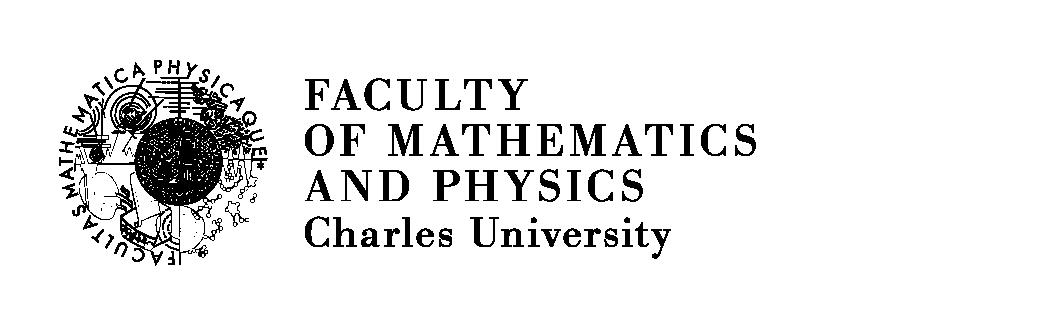
\includegraphics[width=166mm]{../img/logo-en.pdf}}}

\vspace{-8mm}
\vfill

{\bf\Large MASTER THESIS}

\vfill

{\LARGE Vojt\v{e}ch Hude\v{c}ek}

\vspace{15mm}

{\LARGE\bfseries{Exploiting user's feedback to improve pronunciation of TTS systems}}

\vfill

Institute of Formal and Applied Linguistics \\
Faculty of Mathematics and Physics \\
Charles University in Prague \\

\vfill

\begin{tabular}{rl}

Supervisor of the master thesis: & doc. Ing. Zden\v{e}k \v{Z}abokrtsk\'{y}, Ph.D. \\
\noalign{\vspace{2mm}}
Study programme: & Informatics \\
\noalign{\vspace{2mm}}
Study branch: & Artificial Intelligence \\
\end{tabular}

\vfill

% Zde doplňte rok
Prague 2017

\end{center}

\newpage

%%% Here should be a bound sheet included -- a signed copy of the "master
%%% thesis assignment". This assignment is NOT a part of the electronic
%%% version of the thesis. DO NOT SCAN.

%%% A page with a solemn declaration to the master thesis

\openright
\hypersetup{pageanchor=true}
\pagestyle{plain}
\pagenumbering{roman}
\vglue 0pt plus 1fill

\noindent
I declare that I carried out this master thesis independently, and only with the cited
sources, literature and other professional sources.

\medskip\noindent
I understand that my work relates to the rights and obligations under the Act No.~121/2000 Sb.,
the Copyright Act, as amended, in particular the fact that the Charles
University has the right to conclude a license agreement on the use of this
work as a school work pursuant to Section 60 subsection 1 of the Copyright Act.

\vspace{10mm}

\hbox{\hbox to 0.5\hsize{%
In ........ date ............	% FIXME!
\hss}\hbox to 0.5\hsize{%
signature of the author
\hss}}

\vspace{20mm}
\newpage

%%% Mandatory information page of the thesis

\openright

\vbox to 0.5\vsize{
\setlength\parindent{0mm}
\setlength\parskip{5mm}

Title:
Exploiting user's feedback to improve pronunciation of TTS systems

Author:
Bc. Vojt\v{e}ch Hude\v{c}ek

\DeptType:
\Department

Supervisor:
doc. Ing. Zden\v{e}k \v{Z}abokrtsk\'{y}, Ph.D, Institute of Formal and Applied Linguistics

Abstract:
Although spoken dialogue systems have greatly improved, they still cannot handle communications involving unknown topics and are very fragile. We will investigate methods that can improve spoken dialogue systems by correcting or even learn the pronunciation of unknown words. This is a crucial step to provide better user experience, since for example mispronounced proper nouns are highly undesirable. Incorrect pronunciation is caused by imperfect phonetic representation, typically phonetic dictionary. We aim to detect incorrectly pronounced words by exploiting user's feedback as well as using prior knowledge of the pronunciation and correct the transcriptions accordingly. Furthermore, the learned phonetic transcriptions can be used to improve speech recognition module by refining its models. Extracting correct pronunciations benefits both speech-recognition and text-to-speech components of the dialogue systems.

Keywords:
text-to-speech, automatic speech recognition, user's response, phonetic dictionary, machine learning, mel cepstral distortion

\vss}

\newpage

%%% Dedication

\openright

\noindent
\Dedication

\newpage

\openright
\pagestyle{plain}
\pagenumbering{arabic}
\setcounter{page}{1}
